\section{Solution analysis}
After a high level discussion about the characteristics of the solution proposed by this work, now it is time to make an additional step in the road that leads to the concretization of a working system that realizes such idea.

Here, the Domain will be explored, clarifying concepts and nomenclatures in order to uniquely identify the building blocks needed to move forward.
Then, use cases will be discussed, explaining what the system needs to do, seen from the point of view of the actors interacting with it.
Finally, the requirements will be presented, aiming to provide a clear set of criteria to satisfy for a system that wants to use the Transparent scheduling model over heterogeneous devices.

\subsection{Domain}
TODO

\subsection{Use cases}
TODO

\begin{figure}[!ht]
    \centering
    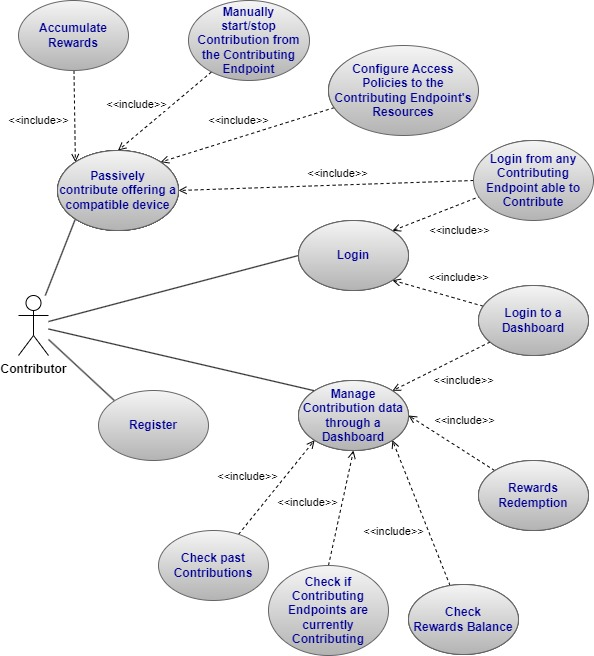
\includegraphics[width=\linewidth]{document/chapters/chapter_5/images/contributor_use_cases.jpg}
    \caption{Contributor's use cases diagram}
    \label{fig:use_cases_contributor}
\end{figure}

\begin{figure}[!ht]
    \centering
    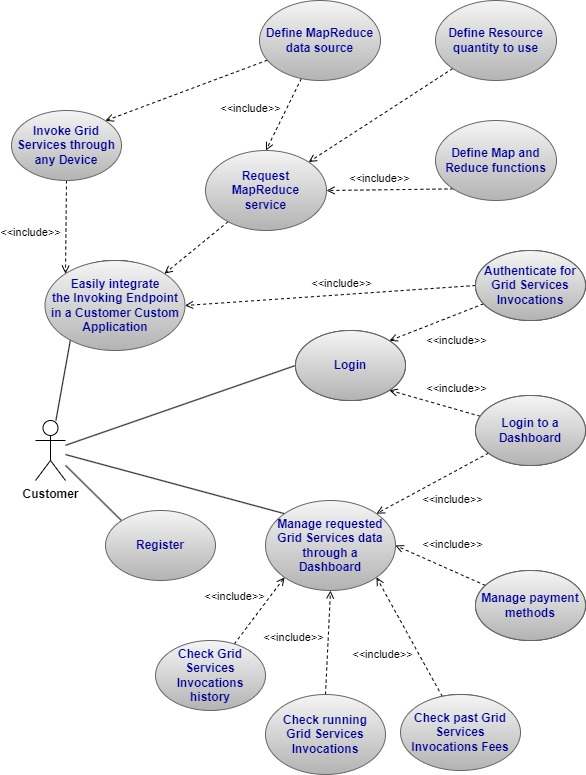
\includegraphics[width=\linewidth]{document/chapters/chapter_5/images/customer_use_cases.jpg}
    \caption{Customer's use cases diagram}
    \label{fig:use_cases_customer}
\end{figure}

\subsection{Requirements}
TODO